\chapter{Características topológicas de los grafos de procesos}
\addcontentsline{toc}{chapter}{Características topológicas de los grafos de procesos}

Teniendo en mente que la finalidad última de este trabajo es encontrar indicadores del progreso de los alumnos y la detección precoz de aquellos grupos con problemas para que el profesor pueda proporcionarles ayuda y orientación, se han obtenido medidas de rendimiento sobre los procesos minados. Se tratarán de funciones \emph{off-the-shelf} genéricas sobre grafos, lo que permitiría aplicar los resulados aquí obtenidos en otras plataformas educativas.

Así pues, se han definido dos métricas distintas: el Laplaciano (\emph{Laplacian}), que usará el análisis espectral de grafos, y la heurística \emph{DAG}, que trata de determinar cómo de balanceados están los nodos de un grafo dirigido acíclico.

\subsection{El Laplaciano (Laplacian)}

En primer lugar, empezamos analizando el \emph{Learning Path} de los grupos para tener una idea de los problemas por los que ha ido navegando durante toda la práctica. En la Figura Figura \ref{fig:DBA1516P2GG} podemos ver el recorrido que hizo el grupo \texttt{DBA1920P2GG}. No obstante, para el cálculo de este coeficiente se usará un grafo de mayor complejidad, en el que se subdividen los estados en \texttt{Pi OK} o \texttt{Pi FAIL} dependiendo del milestone alcanzado (\texttt{OK} indica que se ha resuelto problema). En la Figura \ref{fig:DBA1516P2GG_states} se muestra este nuevo grupo para el grupo de prácticas que estamos considerando.

\begin{figure}[H]
\centering
\subfloat[Grafo que muestra la exploración de los problemas que ha realizado.]{\label{fig:DBA1516P2GG}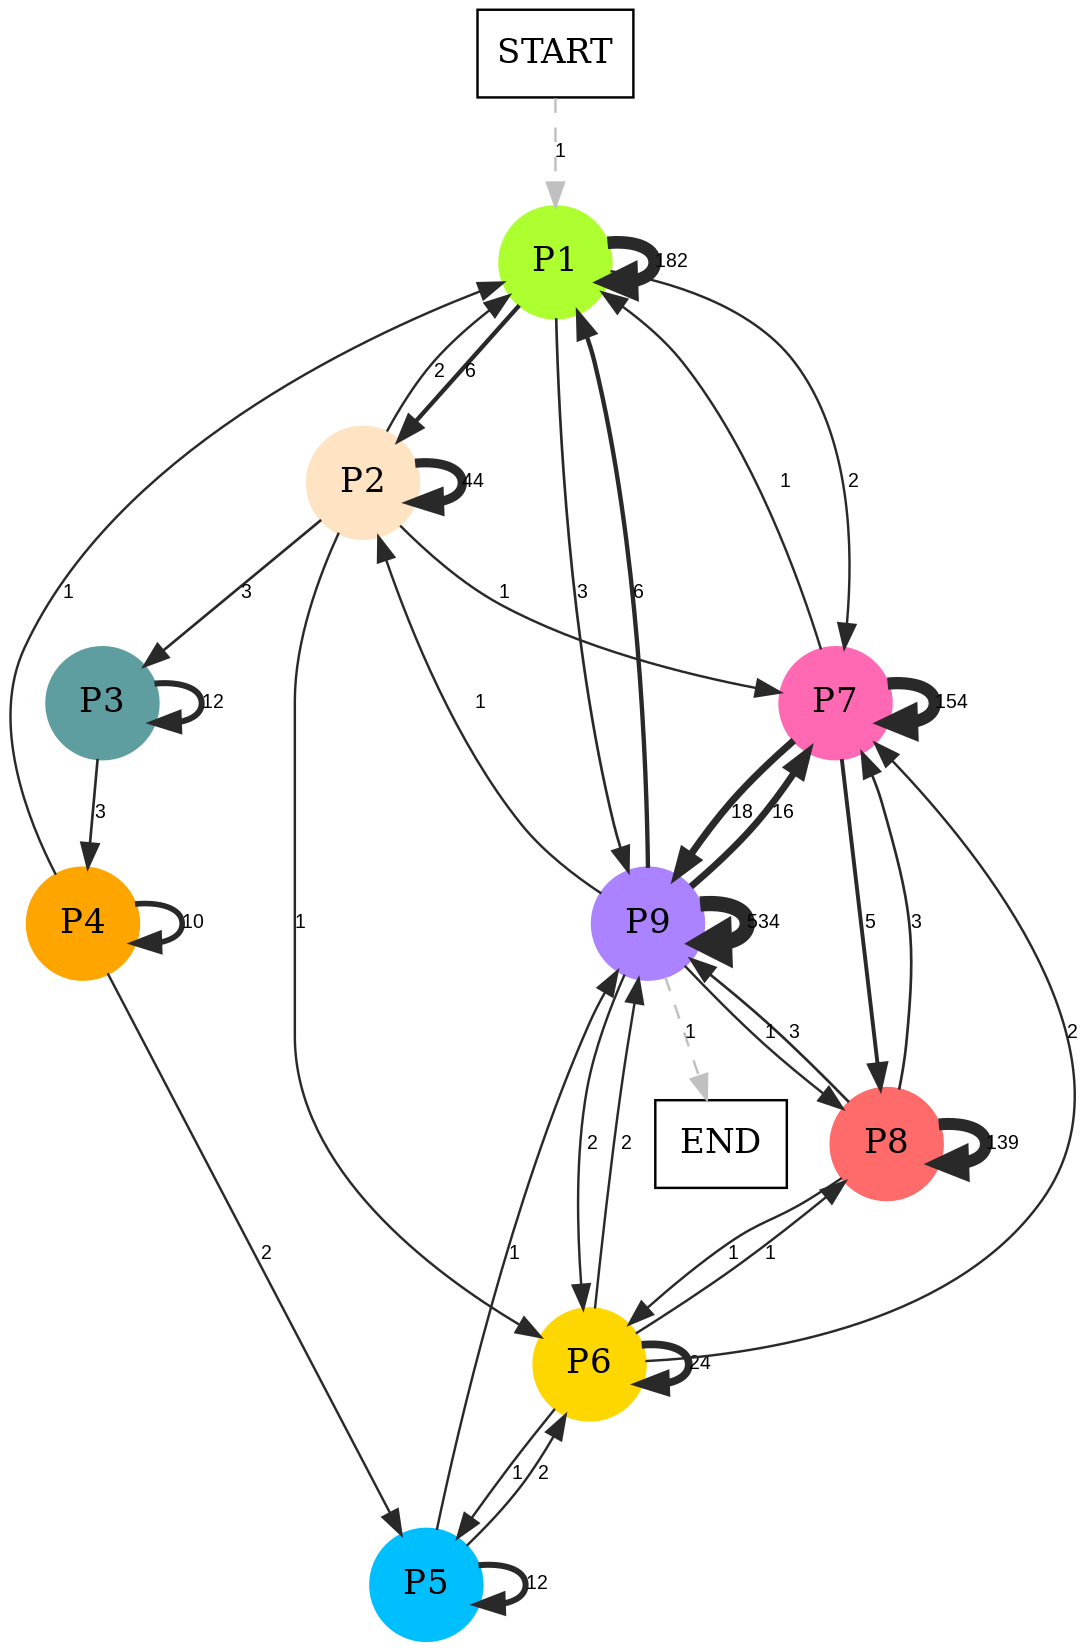
\includegraphics[width=0.47\textwidth]{DBA1516P2GG.png}}\qquad
\subfloat[Grafo que muestra la exploración de los problemas, considerando si un problema ha sido resuelto (\texttt{OK}) o no (\texttt{FAIL}).]{\label{fig:DBA1516P2GG_states}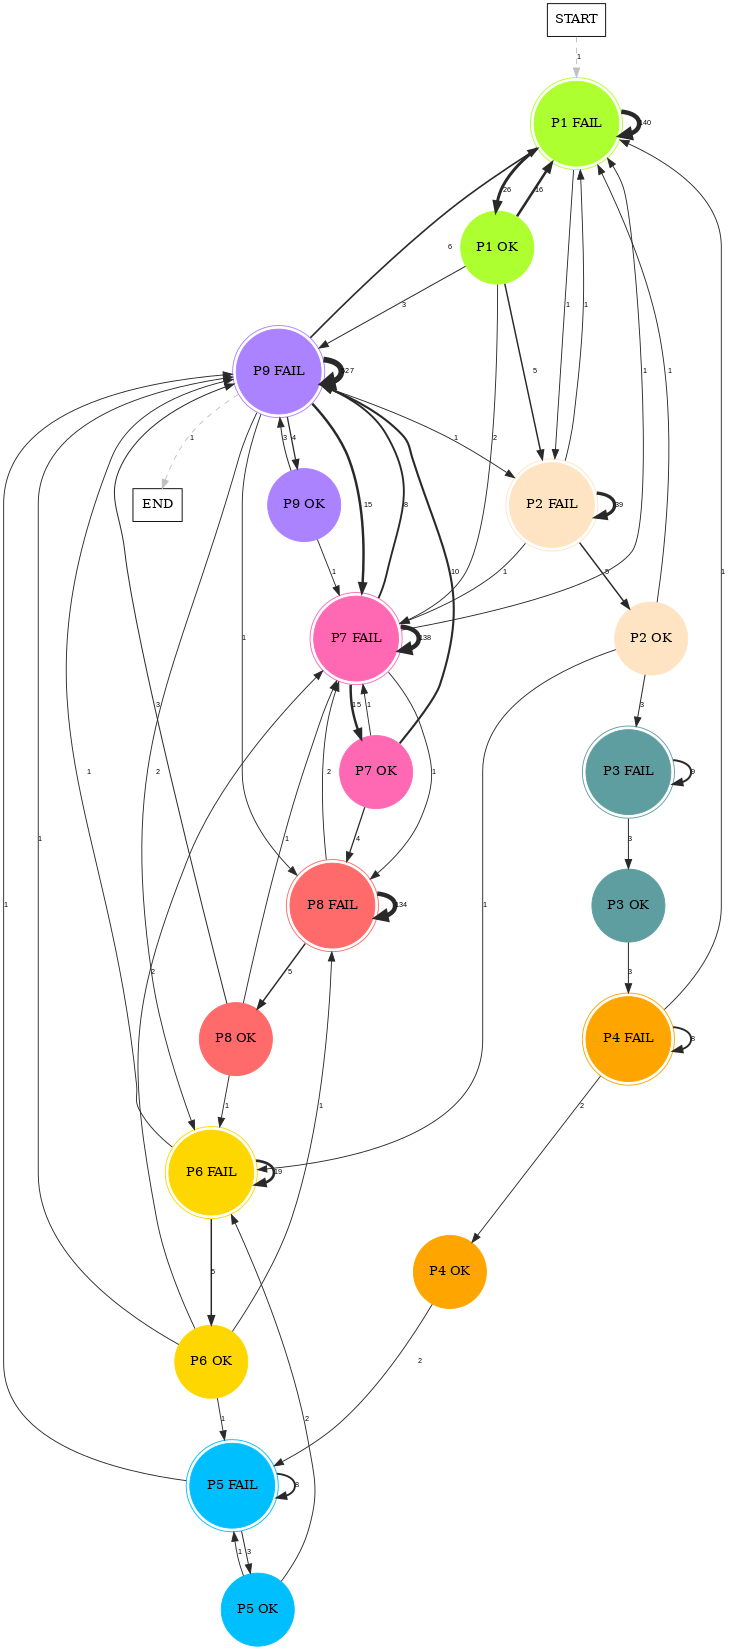
\includegraphics[width=0.47\textwidth]{DBA1516P2GG_states.png}}
\caption{Leaning Path del grupo de prácticas \texttt{DBA1516P2GG}.}
\label{fig:laplacian}
\end{figure}